% ---
% Capa
% ---
\imprimircapa
% ---

% ---
% Folha de rosto
% (o * indica que haverá a ficha bibliográfica)
% ---
\imprimirfolhaderosto*
% ---

% ---
% Inserir a ficha bibliografica
% ---
% http://ficha.bu.ufsc.br/
\begin{fichacatalografica}
	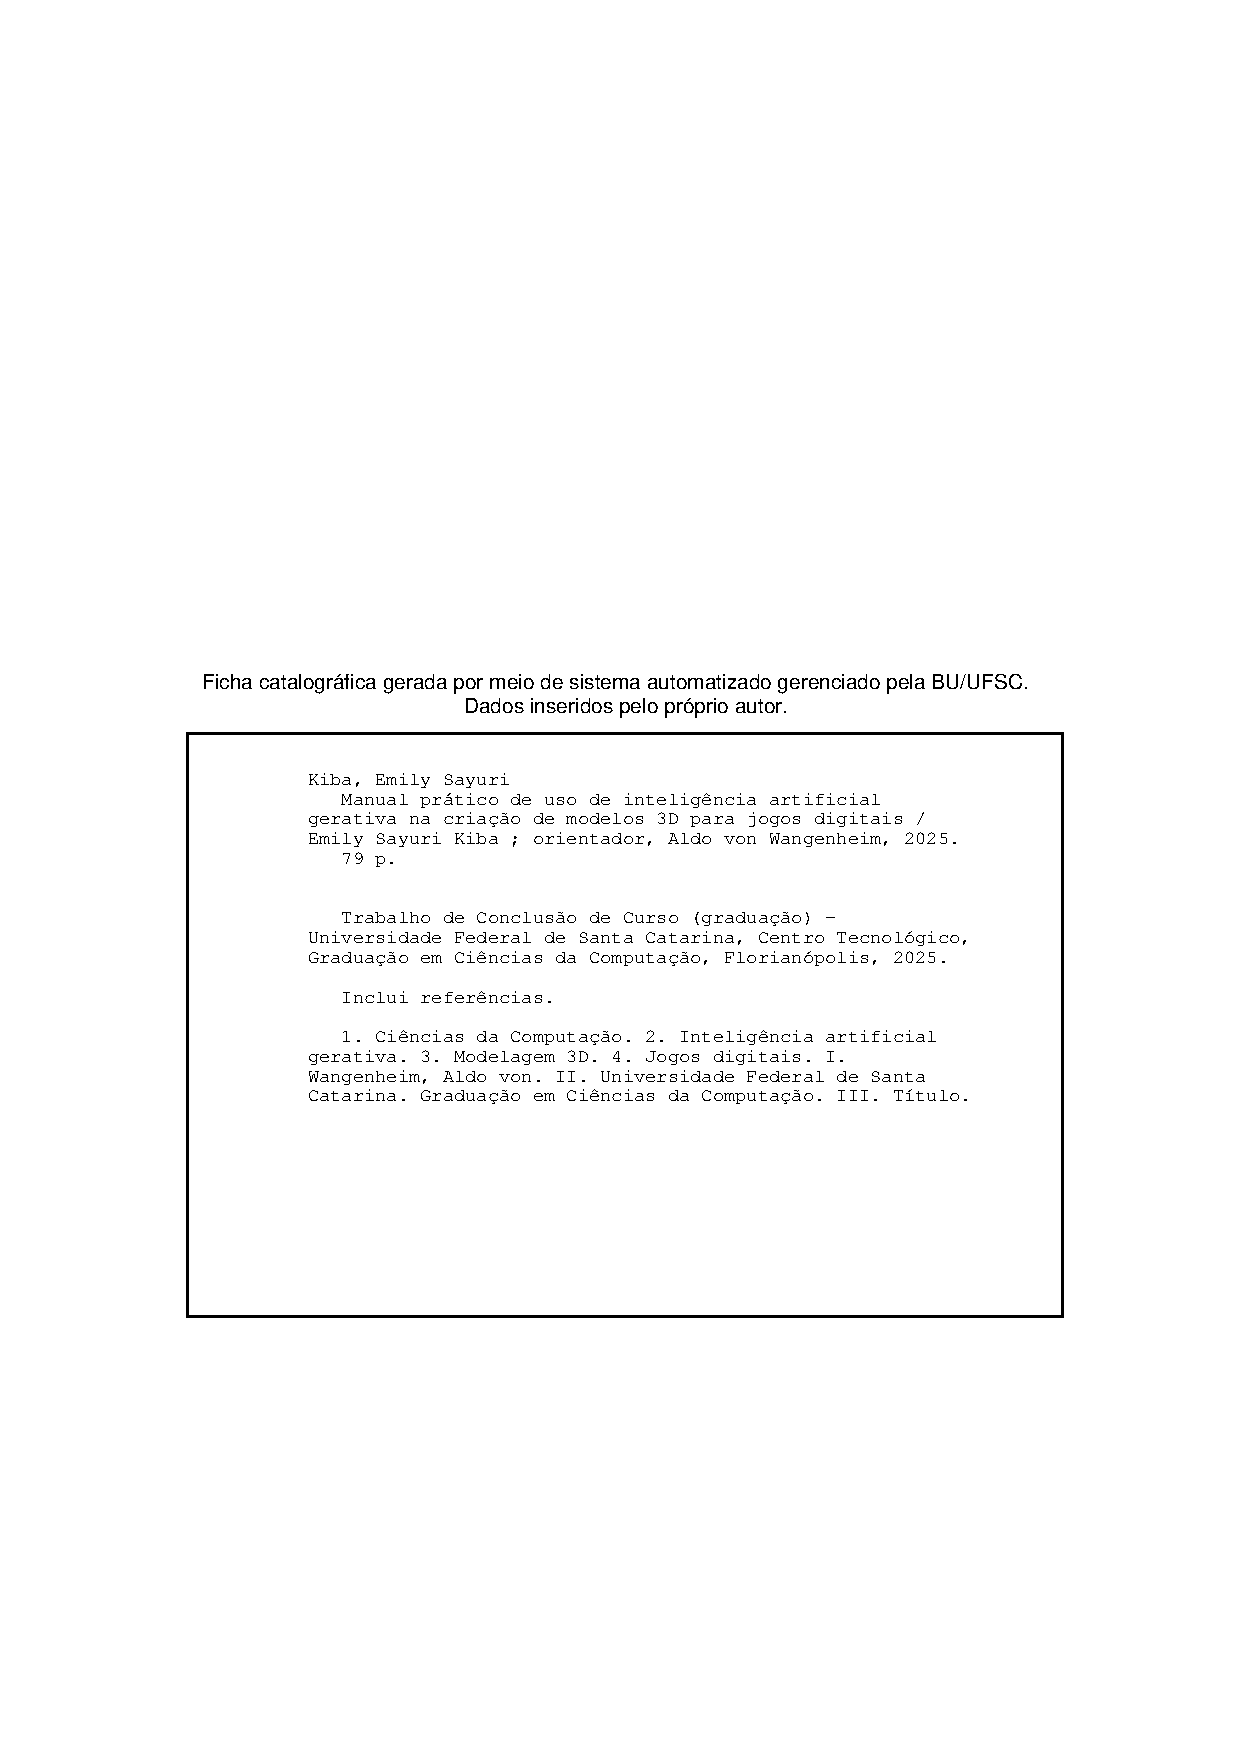
\includepdf{beforetext/Ficha_Catalografica.pdf}
\end{fichacatalografica}
% ---

% ---
% Inserir folha de aprovação
% ---
\begin{folhadeaprovacao}
	\OnehalfSpacing
	\centering
	\imprimirautor\\%
	\vspace*{10pt}		
	\textbf{\imprimirtitulo}%
	\ifnotempty{\imprimirsubtitulo}{:~\imprimirsubtitulo}\\%
	%		\vspace*{31.5pt}%3\baselineskip
	\vspace*{\baselineskip}
	%\begin{minipage}{\textwidth}
	% ~do~\imprimirprograma~do~\imprimircentro~da~\imprimirinstituicao~para~a~obtenção~do~título~de~\imprimirformacao.
	Este~\imprimirtipotrabalho~foi julgado adequado para obtenção do Título de “\imprimirformacao” e aprovado em sua forma final pelo~\imprimirprograma. \\
		\vspace*{\baselineskip}
	\imprimirlocal, \imprimirdata. \\
	\vspace*{2\baselineskip}
	\assinatura{\OnehalfSpacing\imprimircoordenador \\ \imprimircoordenadorRotulo~do Curso}
	\vspace*{2\baselineskip}
	\textbf{Banca Examinadora:} \\
	\vspace*{\baselineskip}
	\assinatura{\OnehalfSpacing\imprimirorientador \\ \imprimirorientadorRotulo}
	%\end{minipage}%
	\vspace*{\baselineskip}
	\assinatura{Prof. Flávio Andaló, Dr.\\
	Avaliador \\
	Universidade Federal de Santa Catarina}
	\vspace*{\baselineskip}
	\assinatura{Eduardo Beckhauser.\\
	Avaliador \\
	Universidade Federal de Santa Catarina}



\end{folhadeaprovacao}
% ---

% % ---
% % Dedicatória
% % ---
% \begin{dedicatoria}
% 	\vspace*{\fill}
% 	\noindent
% 	\begin{adjustwidth*}{}{5.5cm}     
% 		Este trabalho é dedicado aos meus colegas de classe e aos meus queridos pais.
% 	\end{adjustwidth*}
% \end{dedicatoria}
% % ---

% ---
% Agradecimentos
% ---
\begin{agradecimentos}
	Agradeço à minha mãe, Miyuki, e ao meu pai, Takuma, por sempre me apoiarem e me proporcionarem oportunidades para chegar até aqui. Obrigada por acreditarem em mim e me incentivarem, tudo isso sem pressão, com paciência e muito carinho.

	Aos professores do curso de Ciências da Computação, que me proporcionaram tanto conhecimento. Principalmente o professor Aldo, pela orientação, oportunidades e contribuições valiosas ao longo do meu TCC. Agradeço também ao professor Flávio, que me forneceu a modelagem da Ilha de Anhatomirim, essencial para o desenvolvimento do meu TCC. A base fornecida serviu como ponto de partida para a criação do jogo, permitindo realizar alterações e adaptações que enriqueceram o projeto final.

	Ao meu namorado, Rafael, por estar no meu lado me apoiando e aliviando minha ansiedade e o estresse. Pelos momentos de diversão e paz que me permitiram respirar e recarregar as energias, pelas nossas "sessões de MasterChef" cozinhando juntos e rindo, e pelas discussões sobre filmes.

	Aos meus três gatos – Mei, Cookie e Low – por estarem sempre dormindo de forma tão confortável que me dava vontade de abandonar tudo e deitar junto. Ou por me lembrarem que era hora de levantar para servir comida.

	À minha prima, que durante a sua gradução na UFSC dividiu comigo tantos momentos do dia a dia, agradeço pela companhia e pelas conversas em casa. Aos meus avôs, que apareciam para visitar e alegrar o ambiente. Em especial à minha avó, que sempre ajudou nas tarefas da casa, apesar de gostar de me contar muitas fofocas repetidas em todos os momentos, tornou a casa cheio de risadas. 

	Agradeço também aos meus amigos da Ciências da Computação – Eric, Bruno, Gabriela, Gabriel, Julien, Samantha e Marco – pelos inúmeros momentos de diversão, risadas e experiências inesquecíveis. Pelas conversas sobre matérias e professores, e pelos roles como karaokês, trilhas e aniversários, que tornaram o curso muito mais leve e divertido.

	Especialmente o Marco, que conheci no início do curso, durante a pandemia, e que sempre foi meu parceiro de trabalho confiável. Enfrentamos várias madrugadas e trabalhos complicados, mas sobrevivemos junto. 

	Ao Gabriel, mesmo tendo nos conhecido nos últimos dois anos, nossa amizade parece de longa data. As conversas que nunca têm fim – sobre estudos, nossos hiperfocos, discussões animadas, filmes e séries – tornaram a reta final do curso muito mais divertida e significativa. 

	Por fim, agradeço a todos que, de alguma forma, fizeram parte desta caminhada. Cada gesto de apoio, palavra de incentivo, conversa e risada contribuíram para que este trabalho se tornasse realidade.

\end{agradecimentos}
% ---

% ---
% Epígrafe
% ---
% \begin{epigrafe}
% 	\vspace*{\fill}
% 	\begin{flushright}
% 		\textit{``Texto da Epígrafe.\\
% 			Citação relativa ao tema do trabalho.\\
% 			É opcional. A epígrafe pode também aparecer\\
% 			na abertura de cada seção ou capítulo.\\
% 			Deve ser elaborada de acordo com a NBR 10520.''\\
% 			(Autor da epígrafe, ano)}
% 	\end{flushright}
% \end{epigrafe}
% ---

% ---
% RESUMOS
% ---

% resumo em português
\setlength{\absparsep}{18pt} % ajusta o espaçamento dos parágrafos do resumo
\begin{resumo}
	\SingleSpacing
	Este trabalho explora a aplicação de Inteligência Artificial (IA) gerativa, especificamente o Stable Diffusion, na área de modelagem 3D e sua integração no contexto de jogos. O estudo tem como foco a criação de manual prático detalhado, demonstrando como a IA gerativa pode ser utilizada tanto para gerar ideias e conceitos visuais para modelos 3D quanto para a criação direta de malhas e texturas tridimensionais. Dessa forma, o trabalho evidencia o potencial da IA em agilizar o processo de modelagem 3D, simplificando-o ao integrar a IA como uma ferramenta de suporte à criação, tornando-o mais acessível especialmente para usuários sem experiência prévia em modelagem, e contribuindo para a criatividade e eficiência na produção de ativos digitais para jogos.
	
	\textbf{Palavras-chave}: Inteligência Artificial Gerativa. Stable Diffusion. Modelagem 3D. Game Engine.
\end{resumo}

% resumo em inglês
\begin{resumo}[Abstract]
	\SingleSpacing
	\begin{otherlanguage*}{english}
		This work explores the application of Generative Artificial Intelligence (AI), specifically Stable Diffusion, in 3D modeling and its integration into the context of games. The study presents a detailed practical manual demonstrating how generative AI can be used both to generate visual ideas and concepts and to directly create 3D meshes and textures. In doing so, it highlights the potential of AI to streamline and simplify the 3D modeling process, integrating it as a supportive tool for creation, making it accessible to users without prior experience and enhancing creativity and efficiency in the production of digital assets for games.
		
		\textbf{Keywords}: Generative Artificial Intelligence. Stable Diffusion. 3D Modeling. Game Engine.
	\end{otherlanguage*}
\end{resumo}

%% resumo em francês 
%\begin{resumo}[Résumé]
% \begin{otherlanguage*}{french}
%    Il s'agit d'un résumé en français.
% 
%   \textbf{Mots-clés}: latex. abntex. publication de textes.
% \end{otherlanguage*}
%\end{resumo}
%
%% resumo em espanhol
%\begin{resumo}[Resumen]
% \begin{otherlanguage*}{spanish}
%   Este es el resumen en español.
%  
%   \textbf{Palabras clave}: latex. abntex. publicación de textos.
% \end{otherlanguage*}
%\end{resumo}
%% ---

{%hidelinks
	\hypersetup{hidelinks}
	% ---
	% inserir lista de ilustrações
	% ---
	\pdfbookmark[0]{\listfigurename}{lof}
	\listoffigures*
	\cleardoublepage
	% ---
	
	% ---
	% inserir lista de quadros
	% ---
	% \pdfbookmark[0]{\listofquadrosname}{loq}
	% \listofquadros*
	% \cleardoublepage
	% ---
	
	% ---
	% inserir lista de tabelas
	% ---
	\pdfbookmark[0]{\listtablename}{lot}
	\listoftables*
	\cleardoublepage
	% ---
	
	% ---
	% inserir lista de abreviaturas e siglas (devem ser declarados no preambulo)
	% ---
	\imprimirlistadesiglas
	% ---
	
	% ---
	% inserir lista de símbolos (devem ser declarados no preambulo)
	% ---
    % \imprimirlistadesimbolos
	% ---
	
	% ---
	% inserir o sumario
	% ---
	\pdfbookmark[0]{\contentsname}{toc}
	\tableofcontents*
	\cleardoublepage
	
}%hidelinks
% ---